\documentclass{beamer}
%[aspectratio=169]   \usepackage[czech]{babel}
\usepackage{apo-lecture}
\usepackage{pdfpages}
\usepackage{pdfcomment}
\usepackage{listings}
\usepackage{array,multirow}

\subtitle{Lekce 02. Reprezentace čísel}
\author{Petr Štěpán\\ \small\texttt{stepan@fel.cvut.cz}}
\begin{document}

\maketitle

\section{Operace s celými čísly}

\begin{frame}
\frametitle{Opakování}
V minulé lekci jsme měli:
\begin{itemize}
\item Reprezentace bitu pomocí napětí
\item Reprezentace bajtů jako více paralelních vodičů, každý s hodnotou jednoho bitu
\item Sčítání dvou celých kladných čísel
\item Posun celých čísel (násobení, nebo dělení mocninou 2)
\end{itemize}

Dnes:
\begin{itemize}
\item Rozsahy celých čísel a ukládání do paměti
\item Násobení a dělení celých kladných čísel 
\item Reprezentace záporných čísel a operace s nimi
\item Přetečení sčítání a odčístání
\item Reálná čísla
\end{itemize}

\end{frame}


\begin{frame}
\frametitle{Kladná čísla}
Reprezentace celých kladných čísel

V jazyce C jsou typy (podle normy ISO/IEC 9899:TC3):
\begin{tabular}{|l|r|r|c|}\hline
typ & min & max & počet bajtů\\ \hline
unsigned char & 0 & 255 & 1 \\ \hline
unsigned short & 0 & 65 535 & 2 \\ \hline 
unsigned long & 0 & 4 294 967 295 & 4 \\ \hline
unsigned long long & 0 & 18 446 744 073 709 551 615 & 8 \\ \hline
\end{tabular}

\begin{itemize}
\item Norma není vždy dodržována, \texttt{unsigned int} by měl mít jen 2 bajty, ale většinou má 4 bajty (GNU, MS C).
\item Pokud chcete mít jistotu, musíte si pro cílovou platformu zjistit rozsah pomocí příkazu např. \texttt{sizeof(int)}
\end{itemize}

\end{frame}


\begin{frame}
\frametitle{Kladná čísla}
V zápis konstant v jazyce C v soustavě:
\begin{itemize}
\item desítkové -- nesmí začínat 0 kromě 0
\item osmičkové -- začíná 0
\item hexadecimální -- začíná 0x
\item binární -- začíná 0b (pouze GNU překladač)
\end{itemize}
\bigskip
Příklad: 252 == 0xfc == 0374 == 0b11111100
\bigskip

Poznámka: Podle hexadecimálního zápisu zjistíte velikost čísla v bajtech, např. 0x123456 se vejde do tří bajtů.
\end{frame}


\begin{frame}
\frametitle{Kladná čísla - uložení v paměti}

\begin{itemize}
\item Paměť počítače pracuje s bajty
\item Historicky vzniklo několik možností uložení čísel do paměti.
\end{itemize}

Jak lze tedy uložit číslo 0x12345678 do paměti:
\begin{tabular}{|c|c|c|}\hline
adresa & Big-endian & Little-endian \\ \hline
400 & 0x12 & 0x78 \\ \hline
401 & 0x34 & 0x56 \\ \hline
402 & 0x56 & 0x34 \\ \hline
403 & 0x78 & 0x12 \\ \hline
\end{tabular}

\begin{itemize}
\item Procesory Intel zavedly little-endian, procesory Motorola zavedly big-endian.
\item Je to důležité, když získáte například přes internet data po bajtech, musíte definovat, jaká čísla reprezentují
\item RISC V - jsou little-endian, MIPS - big-endian
\item Bitcoin - DER signatures big-endian, transaction hash little-endian
\end{itemize}
\end{frame}

\begin{frame}[fragile]
\frametitle{Kladná čísla - kvíz}
\begin{lstlisting}[language={C},columns=flexible]
#include <stdio.h>
int main() {
  unsigned char p[] = {0,0,0,0};
  *(int*)p=10;
  printf("%02x,%02x,%02x,%02x\n", p[0],p[1],p[2],p[3]);
}
\end{lstlisting}

Co bude výstupem tohoto programu na procesorech Intel?
\begin{itemize}
\item[A] nic, program nelze přeložit
\item[B] náhodný výstup, p  nelze přetypovat na *int
\item[C] 0a,00,00,00 
\item[D] 00,00,00,0a
\end{itemize}
\end{frame}



\begin{frame}
\frametitle{Násobení celých čísel}

Stejný princip násobení, jak jste se ho naučili na základní škole pro desítkovou soustavu:
\begin{columns}
\begin{column}{0.4\textwidth}
\texttt{\phantom{xxx}153}\\
\texttt{\phantom{xxx}*45}\\
\vspace{-8pt}
\rule[0]{1.5cm}{0.1pt}\\
\texttt{\phantom{xxx}765}\\
\texttt{\phantom{xx}612 }\\
\vspace{-8pt}
\rule[0]{1.5cm}{0.1pt}\\
\texttt{\phantom{xx}6885}\\
\end{column}
\hfill
\begin{column}{0.4\textwidth}
\texttt{\phantom{xxxxxx}10011001}\\
\texttt{\phantom{xxxxxxx}*101101}\\
\vspace{-8pt}
\rule[0]{3cm}{0.4pt}\\
\texttt{\phantom{xxxxxx}10011001}\\
\texttt{\phantom{xxxxx}00000000}\\
\texttt{\phantom{xxxx}10011001}\\
\texttt{\phantom{xxx}10011001}\\
\texttt{\phantom{xx}00000000}\\
\texttt{\phantom{x}10011001}\\
\vspace{-8pt}
\rule[0]{3cm}{0.4pt}\\
\texttt{\phantom{x}1101011100101}\\
\end{column}
\end{columns}

\end{frame}

\begin{frame}
\frametitle{Násobení celých čísel}

Podle uvedeného algoritmu můžeme vytvořit náseldující násobičku s posuvným registrem:\\
(A,B 32 bitů, výsledek 64 bitů)
\begin{center}
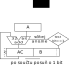
\includegraphics[width=0.5\textwidth]{multiplier-seq.pdf}
\end{center}
\begin{itemize}
\item Výsledek je ve dvou registrech AC a B 
\item Pomalé, už sčítání je náročné, nyní 32 nebo 64 sčítání.
\end{itemize}
\end{frame}


\begin{frame}
\frametitle{Rychlé násobení - Wallace tree}

Jak to zrychlit - odložené carry (Carry Save Adder).\\
Jak nejrychleji spočítat součet čtyř 32-bitových čísel:\\
\begin{columns}
\begin{column}{0.35\textwidth}
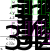
\includegraphics[width=1.0\textwidth]{wallace-tree.pdf}
\end{column}
\hfill
\begin{column}{0.65\textwidth}
\begin{itemize}
\item Sečteme paralelně p=w+x a q=y+z a potom p+q -- trvá dlouho, nejméně doby dvou plných součtů
\item Odložíme carry (nebudeme carry propagovat, jen v posledním kroku):
\begin{itemize}
\item 1. krok použijeme Full adder a sečteme vždy bity $w_i+x_i+y_i = c'_ip_i$
\item 2. krok použijeme Full adder a sečteme vždy bity $p_i+c'_{i-1}+z_i = c_iq_i$
\item 3. krok použijeme normální sčítačku 32-bitových čísel ($s_0=q_0$, $c'_32$ připojíme ke $q$)
\end{itemize}
\end{itemize}
\end{column}
\end{columns}
\end{frame}

\begin{frame}
\frametitle{Rychlé násobení - Wallace tree}

Použijeme předchozí princip na co nejrychlejší součet 32 nebo 64 různých čísel:
\begin{columns}
\begin{column}{0.6\textwidth}
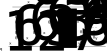
\includegraphics[width=1.0\textwidth]{wallace-tree2.pdf}
\end{column}
\hfill
\begin{column}{0.4\textwidth}
\begin{itemize}
\item Součiny jsou jednoduché: $x_iy_j=x_i$~\texttt{and}~$y_j$
\item Nejtěžší je sečíst prostřední sloupec 64 jednobitových čísel
\end{itemize}
\end{column}
\end{columns}

\end{frame}

\begin{frame}[shrink=5]
\frametitle{Rychlé násobení - Wallace tree}

Když se podíváme jen na prostřední nejdelší sloupec:
\begin{center}
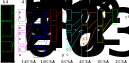
\includegraphics[width=0.8\textwidth]{wallace-tree3.pdf}
\end{center}

\begin{itemize}
\item Vydíme, že za 8 kroků sčítaček, tedy 16 zpoždění hradel nám zbývá sečíst dva bity
\item Vpravo od tohoto sloupce je již vše sečteno a již se i propagovali všechny carry
\item Zbývá sečíct dvě 64-bitová čísla (součty a carry), což se dá stihnout také za 16 zpoždění hradel
\item Výsledek - vynásobíme dvě čísla za cenu doby odpovídajícíc dvou součtům
\end{itemize}

\end{frame}


\begin{frame}
\frametitle{Dělení celých čísel}

Dělení lze zkonstruovat podobně, jako jste se učili na základní škole:
\bigskip
\begin{columns}
\begin{column}{0.4\textwidth}
\texttt{\phantom{-}240:11=21}\\
\texttt{-22}\\
\vspace{-8pt}
\rule[0]{1cm}{0.1pt}\\
\texttt{\phantom{xx}20}\\
\texttt{\phantom{x}-11}\\
\vspace{-8pt}
\rule[0]{1cm}{0.1pt}\\
\texttt{\phantom{xxx}9}\\
\end{column}
\hfill
\begin{column}{0.4\textwidth}
\texttt{\phantom{x}11110000:1011=10101}\\
\texttt{-1011}\\
\vspace{-8pt}
\rule[0]{1cm}{0.4pt}\\
\texttt{\phantom{xx}1000}\\
\texttt{\phantom{xx}10000}\\
\texttt{\phantom{xx}-1011}\\
\vspace{-8pt}
\rule[0]{1.4cm}{0.4pt}\\
\texttt{\phantom{xxxx}1010}\\
\texttt{\phantom{xxxx}10100}\\
\texttt{\phantom{xxxx}-1011}\\
\vspace{-8pt}
\rule[0]{1.8cm}{0.4pt}\\
\texttt{\phantom{xxxxx}1001}\\
\end{column}
\end{columns}
\bigskip
Oba výpočty počítají, že 240 děleno 11 je 21 a zbytek neboli \texttt{240\%11=9}.

\end{frame}


\begin{frame}
\frametitle{Dělení celých čísel}

Dělička počítající \typett{A/B}, A má 64 bitů, B 32 bitů:\\
\begin{columns}
\begin{column}{0.4\textwidth}
číslo A je uloženo ve dvou registrech AC,A\\¨
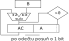
\includegraphics[width=1\textwidth]{divider-seq.pdf}
\end{column}
\hfill
\begin{column}{0.6\textwidth}
\begin{itemize}
\item Výsledek: v registru A je podíl, v registru AC je zbytek -- modulo
\item v posledním kroku je nutné posunout pouze registr A, AC se již neposouvá -- promyslete proč
\item Dělička -- existuje rychlejší algoritmus High Radix Division (je velmi složitý, přesahuje rozsah tohoto předmětu)
\begin{itemize}
\item Odhaduje několik bitů na jednou a pak upřesňuje iteracemi
\item 1994 -- Pentium FDIV bug -- chyba při implementaci algoritmu Sweeney, Robertson, and Tocher (SRT) - odhaduje dva bity
\end{itemize}
\end{itemize}
\end{column}
\end{columns}


\end{frame}


\section{Záporná čísla}

\begin{frame}
\frametitle{Záporná čísla}

Potřebujeme zakódovat znaménko do reprezentace čísla:
\begin{itemize}
\item naivně - vrchní bit bude znaménko
\begin{itemize}
\item Máme 0 a -0, přitom je to stejné číslo
\item Potřebujeme jiný algoritmus na sčítání  
\end{itemize}
\item dvojkový doplněk -- two complement
\begin{itemize}
\item reprezentace x k-bitovým číslem je vlastně $x$ \texttt{mod} $2^k$
\begin{itemize}
\item pro $x\ge0$ je reprezentace $x$
\item pro $x<0$ je reprezentace $2^k-|x|$
\end{itemize}
\item výhoda: sčítání funguje tak, jak jsme si ho navrhli pro všechna čísla, kladná i záporná.
\end{itemize}
\begin{itemize}
\item 8-bitová -1 je \texttt{11111111}
\item 5+(-1) je \texttt{101+11111111=\textcolor{red}{1}00000100}, devátý bit se do reprezentace čísla nevejde, tedy výsledek je \texttt{101+11111111=100}
\end{itemize}
\end{itemize}


\end{frame}

\begin{frame}
\frametitle{Dvojkový doplněk}
\begin{itemize}
\item rozsah čísel reprezentovaných k-bity je $<-2^{k-1}, 2^{k-1}-1>$
\item pro číslo X budeme značit A(X) jeho reprezentaci v dvojkovém doplňku:
\end{itemize}
\vspace{-0.3cm}
\begin{columns}
\begin{column}{0.5\textwidth}
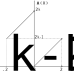
\includegraphics[width=0.9\textwidth]{doplnek-graf.pdf}
\end{column}
\hfill
\begin{column}{0.5\textwidth}
\begin{tabular}{|c|c|}\hline
{\small Binární hodnota}  & {\small Dvojkový doplněk} \\\hline
\textbf{0}0000000 & $0_{(10)}$ \\ \hline
\textbf{0}0000001 & $1_{(10)}$ \\ \hline
... & ... \\\hline
\textbf{0}1111110 & $126_{(10)}$ \\ \hline
\textbf{0}1111111 & $127_{(10)}$ \\ \hline
\textbf{1}0000000 & $-128_{(10)}$ \\ \hline
\textbf{1}0000001 & $-127_{(10)}$ \\ \hline
\textbf{1}0000010 & $-126_{(10)}$ \\ \hline
... & ... \\\hline
\textbf{1}1111101 & $-3_{(10)}$ \\ \hline
\textbf{1}1111110 & $-2_{(10)}$ \\ \hline
\textbf{1}1111111 & $-1_{(10)}$ \\ \hline
\end{tabular}
\end{column}
\end{columns}

\end{frame}

\begin{frame}
\frametitle{Opačné číslo}
\begin{itemize}
\item Protože sčítání funguje s dvojkovým doplňkem, tak nemusíme navrhovat obvod pro odčítání, jednoduše \texttt{A-B} vypočteme jako \texttt{A+(-B)}
\item potřebujeme vymyslet jak získat z \texttt{B} hodnotu \texttt{-B}
\begin{itemize}
\item víme, že záporné $X = 2^k-|X|$
\item pokud znegujeme každý bit, tak je to vlastně $(2^{k-1}-1)-X$, protože $2^{k-1}-1$ je číslo složené z $k$ jedniček
\end{itemize}
\item Výsledný postup je tedy:
\begin{enumerate}
\item znegujte všechny bity čísla $X$
\item k výslednému číslu přičti 1
\end{enumerate}
\end{itemize}

Příklad:\\
\texttt{53=0b00110101} znegováním cifer dostaneme \texttt{-54=0b11001010} po přičtení 1 pak  \texttt{-53=0b11001011}

\end{frame}


\begin{frame}
\frametitle{Odčítání}

Přičteme opačné číslo a je to:

obrázek
\end{frame}

\begin{frame}
\frametitle{Násobení a dělení}

\begin{itemize}
\item pro násobení lze odvodit, že pokud bychom ignorovali znaménko a spočítali A*B, pak musíme výsledek upravit ...
\item moderní násobení a dělení počítá s absolutními hodntami a nakonec určíme znaménko výsledku podle znaménka operandů.
\begin{itemize}
\item nejvyšší bit značí znaménko
\item výpočet opačného čísla je rychlý a levný
\end{itemize}
\end{itemize}
\end{frame}


\begin{frame}
\frametitle{Čísla se znaménkem}
Reprezentace celých čísel

V jazyce C jsou typy:
\begin{tabular}{|l|r|r|c|}\hline
typ & min & max & počet\\
 &  & &  bajtů\\ \hline
char & -128 & 127 & 1 \\ \hline
short & -32 768 & 32 767 & 2 \\ \hline 
long & -2 147 483 648 & 2 147 483 647 & 4 \\ \hline
long long & -9 223 372 036 & 9 223 372 036  & 8 \\ 
 & \phantom{xx} 854 775 808 & \phantom{xx}854 775 807 &  \\ \hline
\end{tabular}

\begin{itemize}
\item Norma C má ve skutečnosti min o 1 větší , kvůli procesorům s jedničkovým doplňkem -- ten se dnes již prakticky nepoužívá
\item Stejně tak \texttt{int} musíte otestovat, zda je 2 bajtový nebo 4 bajtový
\end{itemize}

\end{frame}


\begin{frame}[fragile, shrink=5]
\frametitle{Kvíz}

Uvažujte tento program:
\begin{minted}{c}
#include <stdio.h>
int main() {
  unsigned char a=150u, b=120u, c;
  char sa=-100, sb=-80, sc;
  
  c=a+b;
  sc=sa+sb;
  printf("c=%u sc=%d\n", c, sc);
}
\end{minted}

Co program vytiskne:
\begin{itemize}
\item[A] c=270 sc=-180
\item[B] c=14 sc=-76
\item[C] c=14 sc=76
\item[D] c=-14 sc=-76
\item[E] Numeric error
\end{itemize}
\end{frame}

\begin{frame}
\frametitle{Přetečení}

Přetečení při sčítání kladných čísel:

Pokud se podíváme co se stalo, unsigned char je 8-bitová reprezentace čísel:\\
\texttt{\phantom{x}150 = \phantom{x}1001 0110}\\
\texttt{+120 = \phantom{x}0111 1000}\\
\texttt{\phantom{xx}14 = \phantom{x}0000 1110}\\
\texttt{\phantom{x}270 =1 0000 1110}

Protože se výsledek nevejde do 8-bitů, nejvyšší jednička se ztratí a výsledek je pouze 14.

Pokud to chcete detekovat, máte následující možnosti:
\begin{itemize}
\item C23 bool ckd\_add(type1 *result, type2 a, type3 b) -- součet dvou čísel s detekcí přetečení
\item GNU GCC 5+, Clang 3.8+ \_\_builtin\_add\_overflow(a, b, result) -- obě verze i pro sub a mul
\end{itemize}
\end{frame}

\begin{frame}
\frametitle{Přetečení}

Přetečení při sčítání Záporných čísel.
\end{frame}


\begin{frame}
\frametitle{Jiné reprezentace záporných čísel}

Čísla s posunutou nulou
\end{frame}

\begin{frame}
\frametitle{Počítání s posunutou nulou}

Čísla s posunutou nulou
\end{frame}


\begin{frame}
\frametitle{Jiné reprezentace záporných čísel}

Doplněk jedné

BCD formát
\end{frame}


\section{Reálná čísla}


\begin{frame}
\frametitle{Reálná čísla}

Dvojková reálná čísla

\end{frame}


\begin{frame}
\frametitle{Reálná čísla}

Čísla s pevnou destinnou čárkou

Obdoba čísel s posunutou nulou

Jednoduché sčítání odčístání, složité násobení, dělení
\end{frame}

\begin{frame}
\frametitle{Plovoucí desetinná čárka}

Plovoucí desetinná čárka, floating point numbers

Obdoba dekadického zápisu reálných čísel

\end{frame}

\begin{frame}
\frametitle{IEEE-754}

Základní definice znaménko exponent mantisa (skrytá jednička) 
\end{frame}


\begin{frame}
\frametitle{IEEE-754}

Normalizované, denormalizované čísla

Nekonečna a NaN
\end{frame}

\begin{frame}
\frametitle{IEEE-754}

Porovnání dvou reálných čísel

\end{frame}


\begin{frame}
\frametitle{IEEE-754}

Sčítání dvou reálných čísel

\end{frame}


\begin{frame}
\frametitle{IEEE-754}

Sčítání dvou reálných čísel

\end{frame}

\begin{frame}
\frametitle{IEEE-754}

Násobení dvou reálných čísel

\end{frame}

\begin{frame}
\frametitle{Bonusový bod}

Kvíz s bonusovou otázkou za tuto hodinu.

\end{frame}




\end{document}

